\documentclass{article}
\author{Tyler Compton}
\title{Section 10.1 - 3D Analysis}

\usepackage{graphicx}
\usepackage{float}
\usepackage{amsfonts}
\usepackage{gensymb}
\usepackage{amsmath}
\graphicspath{ {images/} }

\begin{document}

\maketitle
\tableofcontents

\section{Introduction}
Calculus \textrm{III} introduces the concept of 3D space and how it relates to
mathematics. This text discusses 3D coordinates, 3D graphs, planes as they
relate to 3D space, distance between points, vectors, and projection.

\section{Graphs in 3D}
Everyone is familiar with the 2D coordinate graph. How do 3D coordinate graphs
look?

\begin{figure}[H]
	\centering
	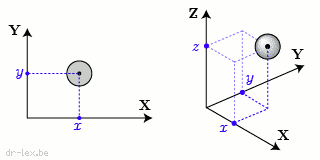
\includegraphics[width=8cm]{2d-vs-3d-planes}
	\caption{Comparison of 2D and 3D planes}
	\label{fig:planes}
\end{figure}
6
As seen in \ref{fig:planes}, the Z axis extends upwards while the X and Y axes
point as if the coordinate plane were placed on the ground.

Two-dimensional space is often referred to as $\mathbb{R}^2$, and three-
dimensional space is referred to as $\mathbb{R}^3$. One could imagine that
four-dimensional space could be called $\mathbb{R}^4$.

\section{Points on Planes}
A point can be said to reside on a ``plane'' if it lines up with two of the
three axes.

\begin{table}[H]
	\centering
	\begin{tabular}{ l c r }
		(2, 3, 5) & $\rightarrow$ & Not on a plane \\
		(2, 3, 0) & $\rightarrow$ & XY Plane \\
		(0, 3, 5) & $\rightarrow$ & YZ Plane \\
		(2, 0, 5) & $\rightarrow$ & XZ Plane \\
	\end{tabular}
\end{table}

As you can see, a point is on a plane if either the X, Y, or Z values are zero.

\section{Distance Between Points in 3D Space}
In a two dimensional coordinate system, distance is given by what's commonly
called the ``distance formula'', which is made from solving for the hypotenuse
using the Pythagorean Theorum.

$$d = \sqrt{(\Delta x)^2 + (\Delta y)^2}$$

As it turns out, distance in a three dimensional coordinate system uses the
same principle. We just need to add the Z component like so:

$$d = \sqrt{(\Delta x)^2 + (\Delta y)^2 + (\Delta z)^2}$$

We can use this to get the magnitude of a three dimensional vector given two
points.

\section{Projection}
If one were to take the point (2, 3, 5) in three dimensional space and remove
the Z component, you would have the point (2, 3, 0). The technical way to
discuss this relationship would be to say that ``the projection of (2, 3, 5) on
the XY plane is (2, 3, 0)'' because the XY plane is what we're left with after
removing the Z component.

Similarly, if one were to remove the Y component from the same point, that new
point would be (2, 0, 5) and you might say that the projection of (2, 3, 5) on
the XZ plane is (2, 0, 5).

Another way to think of projection is to imagine positioning a flashlight over
the plane in question such that the point is in between the flashlight and the
plane. The shadow cast by the point is the position of that point's projection.

\section{Simple Equations in 3D}
Let's look at a simple equation in 2D space. The equation $y=2$ produces a
simple line in $\mathbb{R}^2$.

\begin{figure}[H]
	\centering
	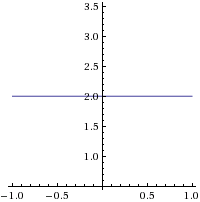
\includegraphics[width=6cm]{y=2-2d}
	\caption{The graph of $y=2$ in $\mathbb{R}^2$}
	\label{fig:y=2-2d}
\end{figure}

What would this graph look like in $\mathbb{R}^3$? Well, in order to come up
with the $\mathbb{R}^2$ graph, we figured out that since x is not in the
formula $y=2$, y will not change for all x. In other words, for all x, $y=2$.

In $\mathbb{R}^3$, we go through the same thought process, except for with the
z value, as well. As with x, z does not appear in our formula, meaning that y
will not change for all z, as well. To bring it all together, for all x and z,
$y=2$. For x in $\mathbb{R}^2$, we expressed this by extending our graph out
for infinity as a straight, level line. In $\mathbb{R}^3$, we do the same thing
for z by extending it infinitely upwards and downwards. This creates what's
referred to as a plane, or a rectangle of infinite width and height that
extends in all directions.

\begin{figure}[H]
	\centering
	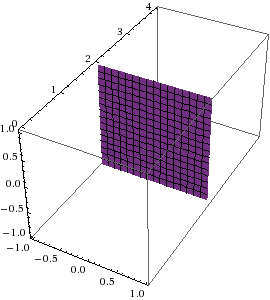
\includegraphics[width=6cm]{y=2-3d}
	\caption{The graph of $y=2$ in $\mathbb{R}^3$}
	\label{fig:y=2-3d}
\end{figure}

Similarly, with the equation $y=x$, we get another plane, this time parellel to
the z axis and tilted $45\degree$ from the x axis.

\begin{figure}[H]
	\centering
	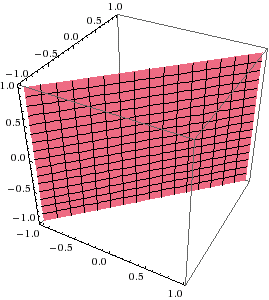
\includegraphics[width=6cm]{y=x-3d}
	\caption{The graph of $y=x$ in $\mathbb{R}^3$}
	\label{fig:y=x-3d}
\end{figure}

You might notice that all of these equations that make planes have variables
with a maximum power of one. This is a good rule of thumb to help you visualize
$\mathbb{R}^3$ equations. This is because, just like in $\mathbb{R}^3$,
variables to the power of one create linear equations. Planes are simply linear
equations in $\mathbb{R}^3$.

Another helpful way to visualize $\mathbb{R}^3$ planar equations is to graph
their x, y, and z intercepts, then draw a rectangle that hits all these
points.

\section{Shapes in 3D}
The standard form for a circle equation is the following:

$$r^2 = (x - j)^2 + (y - k)^2$$

Where r is the radius, j and k are the center coordinates, and x and y are any
point on the circle's edge.

By graphing the equation $9 = x^2 + y^2$, we get the following.

\begin{figure}[H]
	\centering
	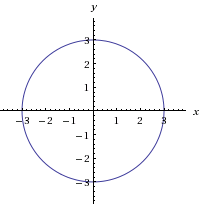
\includegraphics[width=6cm]{circle-radius-3}
	\caption{The graph of a basic circle}
	\label{fig:circle}
\end{figure}

We can also tell by consulting the circle standard form that the radius of the
circle in \ref{fig:circle} has a radius 3 and a center of (0, 0).

If this equation is graphed in $\mathbb{R}^3$, it would follow the same rules
as the linear equations did. Since z is not part of the equation, the equation
will not change for all values of z. The result is an infinite amount of
circles stacked on top and underneath each other. In other words, it makes a
cylinder of infinite height.

\section{3D Shapes in 3D}
Now that we've discussed expressing two-dimensional equations in
$\mathbb{R}^3$, let's move on to graphing true three-dimensional functions with
z as a variable in the equation.

$$x^2 + y^2 = z$$

You might notice that this equation is suspiciously circle-like. The only
difference between this one and the equation we were working with before is
that the radius is z instead of a constant. That would mean that instead of the
shape remaining constant, the circle will grow as the equation moves up the z
axis. On first inspection, you might expect this to make a cone-shaped graph.

\begin{figure}[H]
	\centering
	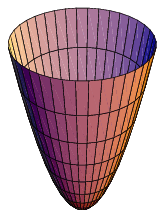
\includegraphics[width=4cm]{paraboloid}
	\caption{The graph of $x^2 + y^2 = z$. Is it what you expected?}
	\label{fig:paraboloid}
\end{figure}

But wait, what's this? That is not the cone we may have expected! Despite
looking linear, the circle's growth is actually parabolic. The shape we've
come up with is not a cone, but a paraboloid. If the equation were
$x^2 + y^2 = z^2$, the graph would be a cone, as expected.

Spheres are a logical extension of the circle formula, much like the 3D
distance formula is an extension of the 2D distance formula. The sphere
equation in standard form is the following:

$$r^2 = (x + j)^2 + (y + k)^2 + (z + l)^2$$

\begin{figure}[H]
	\centering
	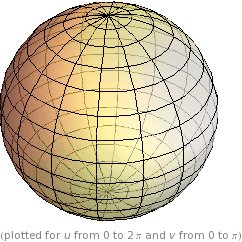
\includegraphics[width=6cm]{sphere}
	\caption{A sphere.}
	\label{fig:sphere}
\end{figure}

Much like with the circle, having a sphere equation in standard form makes it
easy to find the center point and the radius. It would be desirable to convert
sphere equations to standard form if it isn't already.

\section{Completing the Square to Find a Sphere's Standard Form}
The folloiwng is a sphere equation that is not in standard form.

$$x^2 + y^2 + z^2 + 2x - 4y + 10z = 3$$

With this equation, it's unclear how best to convert it to standard form using
conventional methods. Completing the square is very helpful for this purpose.
We will start by consolidating terms with the same variables.

$$x^2 + 2x + y^2 - 4y + z^2 + 10z = 3$$

Then we add and subtract by the coefficient of the non-squared term divided by
two, squared. In other words, for $x^2 + 2x$ we would add
$(\dfrac{2}{2})^2 - (\dfrac{2}{2})^2$.

$$x^2 + 2x + (\dfrac{2}{2})^2 - (\dfrac{2}{2})^2 + y^2 - 4y + (\dfrac{-4}{2})^2 - (\dfrac{-4}{2})^2 + z^2 + 10z + (\dfrac{10}{2})^2 - (\dfrac{10}{2})^2 = 3$$

A quick mind might notice that this does absolutely nothing, mathematically.
You would be right. The reason why we did this is to make a trick we can do a
bit more obvious. Consider the relationship between these two equations:

\begin{tabular}{ l r }
	$(x - h)^2$ \\
	$x^2 - 2xh + h^2$ \\
\end{tabular}

First thing's first, you might notice that these two equations are equivalent.
Secondly, notice that the first and third terms of the second equation are the
first and second terms of the first equation, squared. We're using this
property to do a shortcut by completing the square. We've made $x^2 + 2x$ into
$x^2 + 2x + (\dfrac{2}{2})^2$, which closer resembles the second equation's
format, a de-FOILed equation. Then, we are using the rules we observed to turn
it into a format like the first equation, like so.

$$(x + 1)^2 + (y - 2)^2 + (z + 5)^2 - (\dfrac{2}{2})^2 - (\dfrac{-4}{2})^2 - (\dfrac{10}{2})^2 = 3$$

Then we simply move our risidual fractions over to the radius side of the
equation and we have our sphere form.

\end{document}
